\documentclass[12pt]{article}
%\documentclass[a4paper,14pt]{extarticle} turn on for size 14 font

%general things:
\usepackage[hidelinks]{hyperref} %I dislike the colored boxed hyperlinks. This hides those colored boxes.
\usepackage{enumitem} %for (a) (b) (c) enumeration
\usepackage{fullpage} %sets the margins to 1inch. Turn off for the more restrictive TeX default...
\usepackage{epigraph} %I love epigraphs...
\usepackage{appendix}

%fonts:
\usepackage[T1]{fontenc}
\usepackage{euler} %Thanks to AJ Lawrence for this one
\usepackage{beton} %

\AtBeginDocument
{\DeclareFontShape\encodingdefault{ccr}{bx}{n}{<->sub*cmss/sbc/n}{}%
\DeclareFontShape\encodingdefault{ccr}{bx}{it}{<->sub*cmss/sbc/it}{}%
\DeclareFontShape\encodingdefault{ccr}{bx}{sl}{<->sub*cmss/sbc/sl}{}%
\DeclareFontShape\encodingdefault{ccr}{bx}{sc}{<->sub*cmss/sbc/sc}{}}


\usepackage{aurical} % for Kyle Spratt's dissertation appearance, usse baskervald
%\usepackage{baskervald} %calligraphic font




%math
\usepackage{amsmath}
%this handles numbering according to section/subsection/subsubsection
\numberwithin{equation}{section}

\usepackage{mathabx}
\usepackage{graphicx}
\usepackage{float}
\usepackage{siunitx}
\usepackage{commath}
\usepackage{tkz-euclide} %use mathcha.io for generating beautiful figures in TeX
\usepackage{braket} %quantum
\usepackage{tikzducks}%ducks


%color:
\usepackage{xcolor}

%beautiful boxed equations
\usepackage{empheq}
\usepackage[most]{tcolorbox}
\newtcbox{\maybe}[1][]{%
    nobeforeafter, math upper, tcbox raise base,
    enhanced, colframe=yellow!65!black,
    colback=yellow!15, boxrule=0.75pt,
    #1}
\newtcbox{\love}[1][]{%
    nobeforeafter, math upper, tcbox raise base,
    enhanced, colframe=pink!65!black,
    colback=pink!15, boxrule=0.75pt,
    #1}
\newtcbox{\eq}[1][]{%
    nobeforeafter, math upper, tcbox raise base,
    enhanced, colframe=blue!65!black,
    colback=yellow!10, boxrule=0.75pt,
    #1}
\newtcbox{\correct}[1][]{%
    nobeforeafter, math upper, tcbox raise base,
    enhanced, colframe=green!65!black,
    colback=green!10, boxrule=0.75pt,
    #1}

\newtcbox{\incorrect}[1][]{%
    nobeforeafter, math upper, tcbox raise base,
    enhanced, colframe=red!65!black,
    colback=red!10, boxrule=0.75pt,
    #1}

%text boxes
\newtcolorbox{graytext}[2][%
    enhanced, 
    breakable,
    skin first=enhanced,
    skin middle=enhanced,
    skin last=enhanced,
    ]{colframe=gray!65!black,fonttitle=\bfseries, boxrule=0.75pt, colbacktitle=gray!85!black,enhanced,
attach boxed title to top center={yshift=-2mm},
  title={#2},#1}

\newtcolorbox{bluetext}[2][%
    enhanced, 
    breakable,
    skin first=enhanced,
    skin middle=enhanced,
    skin last=enhanced,
    ]{colframe=blue!65!black,colback=blue!10,fonttitle=\bfseries, boxrule=0.75pt, colbacktitle=blue!85!black,enhanced,
attach boxed title to top center={yshift=-2mm},
  title={#2},#1}

%User-defined commands
%Ordering:
\newcommand{\Order}{\mathcal{O}}
%vector and tensor symbols:
\renewcommand{\vec}[1]{\boldsymbol{#1}}
\newcommand{\tensor}[1]{\underline{\boldsymbol{#1}}} %may need to change to renewcommand. 
\renewcommand{\div}{\boldsymbol{\nabla}\cdot}
\newcommand{\grad}{\boldsymbol{\nabla}} 
\newcommand{\curl}{\boldsymbol{\nabla}\times}
\newcommand{\Laplacian}{\nabla^2}
\newcommand{\dAlambertian}{\Box^2}
\newcommand{\T}{^{\mathsf{T}}}%transpose
%even and odd:
\newcommand{\even}{^{\mathrm{e}}} %even quantity in wavenumber
\newcommand{\odd}{^{\mathrm{o}}} %odd quantity in wavenumber
%micros/meso/macro-related subscripts
\newcommand{\s}{_\mathrm{s}} %scattered quantity subscript

%%%%%%%%%%%%
%%%%%%%%%%%%
%D O C U M E N T        
%%%%%%%%%%%%
%%%%%%%%%%%%
% S T A R T S   
%%%%%%%%%%%%
%%%%%%%%%%%%
% H E R E
%%%%%%%%%%%%
%%%%%%%%%%%%
\title{\textsf{euler} and \textsf{beton} notes template}
\author{Chirag\footnote{\texttt{chiragokani@gmail.com}}} %can use \Fontlukas or \Fontauri for calligraphic font
\date{\today}
\begin{document}
\maketitle
%%%%%%%%%%%%%%%%%%%%%%%%%%%%%%%%
%%%%%%%%%%%%%%%%%%%%%%%%%%%%%%%%
%%%%%%%%%%%%%%%%%%%%%%%%%%%%%%%%
\setlength{\epigraphwidth}{0.31\textwidth}
\epigraph{\Fontlukas A place for everything,\\and everything in its place}{\Fontlukas---Mother}
%%%%%%%%%%%%%%%%%%%%%%%%%%%%%%%%
%%%%%%%%%%%%%%%%%%%%%%%%%%%%%%%%
%%%%%%%%%%%%%%%%%%%%%%%%%%%%%%%%
%In place of an epigraph, one can include images using the tcolorbox package. Uncommented for now, but I like this format.
\iffalse
\begin{tcbraster}[raster columns=3,raster rows=1,raster height= 5.2cm, raster width= \linewidth,
  enhanced,size=small,arc=2mm,colframe=gray!65!black,
  colback=gray!10!white,watermark overzoom=1,fit algorithm=hybrid* ]
\begin{tcolorbox}[rounded corners=northwest,boxrule=0pt,
watermark graphics=lightning.jpeg]\end{tcolorbox} %\tcboxfit{}
\begin{tcolorbox}\textit{you can insert some text here with pictures on either side...}\end{tcolorbox}
\begin{tcolorbox}[rounded corners=northeast,boxrule=0pt,
watermark graphics=jet.jpeg]\end{tcolorbox}
\end{tcbraster}
\fi
%%%%%%%%%%%%%%%%%%%%%%%%%%%%%%%%
%%%%%%%%%%%%%%%%%%%%%%%%%%%%%%%%
%%%%%%%%%%%%%%%%%%%%%%%%%%%%%%%%
\begin{graytext}{Description of notes}
This template formats documents the way I prefer. The description and status of these associated notes is color-coded as \color{cyan}\textit{complete} \color{black} and  \color{magenta}\textit{incomplete}\color{black}.
\begin{enumerate}[label=(\alph*)]
\item \color{cyan}\texttt{blahblah.pdf}: covers blah blah blah \color{black} 
\item \color{magenta}\texttt{blahblahblah.pdf} discusses blah blah blah blah \color{black} 
\end{enumerate}
\end{graytext}
%%%%%%%%%%%%%%%%%%%%%%%%%%%%%%%%
%%%%%%%%%%%%%%%%%%%%%%%%%%%%%%%%
%%%%%%%%%%%%%%%%%%%%%%%%%%%%%%%%
\tableofcontents
%%%%%%%%%%%%%%%%%%%%%%%%%%%%%%%%
%%%%%%%%%%%%%%%%%%%%%%%%%%%%%%%%
%%%%%%%%%%%%%%%%%%%%%%%%%%%%%%%%
\section{Governing equations}
%%%%%%%%%%%%%%%%%%%%%%%%%%%%%%%%
%%%%%%%%%%%%%%%%%%%%%%%%%%%%%%%%
%%%%%%%%%%%%%%%%%%%%%%%%%%%%%%%%
This is a section. Keep in mind that all numbers (if meant to be  mathematical symbols) must appear in the math environment; for example consider 1 vs $1$. If one doesn't like the section/subsection/subsubsection formatting, one can delete these headers as well as the \texttt{\textbackslash tableofcontents}. Here is a centered aligned equation:
\begin{empheq}[box=\eq]{align}
\div \vec{u} + \frac{\partial \rho}{\partial t} &= 0 \label{co}\\
\grad P + \frac{\partial }{\partial t}(\rho \vec{u}) &= 0 \label{mo}
\end{empheq}
%%%%%%%%%%%%%%%%%%%%%%%%%%%%%%%%
%%%%%%%%%%%%%%%%%%%%%%%%%%%%%%%%
%%%%%%%%%%%%%%%%%%%%%%%%%%%%%%%%
\section{Wave equation}
%%%%%%%%%%%%%%%%%%%%%%%%%%%%%%%%
%%%%%%%%%%%%%%%%%%%%%%%%%%%%%%%%
%%%%%%%%%%%%%%%%%%%%%%%%%%%%%%%%
Linearizing equations (\ref{co}) and (\ref{mo}) and combining with an equation of state gives the wave equation of linear acoustics,
\begin{empheq}[box=\correct]{equation*}
\Laplacian P - \frac{1}{c_0^2}\frac{\partial^2 p}{\partial t^2} = \Order(\epsilon^2)
\end{empheq}
This can also be written as 
\begin{equation*}
\dAlambertian p = \Order(\epsilon^2)\,.
\end{equation*}
Here are some \TeX commands I always seem to forget: \texttt{\textbackslash gtrsim, \textbackslash lesssim, \textbackslash stackrel{?}{=}}.
\begin{bluetext}{Concluding thoughts}
Write your conclusions/thoughts here.
\end{bluetext}
%%%%%%%%%%%%%%%%%%%%%%%%%%%%%%%%
%%%%%%%%%%%%%%%%%%%%%%%%%%%%%%%%
%%%%%%%%%%%%%%%%%%%%%%%%%%%%%%%%
\section*{Appendix}
%%%%%%%%%%%%%%%%%%%%%%%%%%%%%%%%
%%%%%%%%%%%%%%%%%%%%%%%%%%%%%%%%
%%%%%%%%%%%%%%%%%%%%%%%%%%%%%%%%
\begin{table}[H]
\centering
\begin{tabular}{ l | l} 
	\textbf{Symbol} & \textbf{Quantity/Operation} \\
	\hline\hline
	$i$ & complex unit\\
	$x$ & scalar\\		
	$\vec{x}$ & column vector\\
	$\hat{x}$ & unit vector in direction of $\boldsymbol{x}$\\
	$\boldsymbol x\T$ & row vector\\
	$\tensor{X}$ & dyadic\\		
	$\tensor{X}^*$ & complex conjugation\\
	$\tensor{X}\T$ & transposition\\
	$\tensor{X}^\dagger$ & Hermitian conjugate\\	
	$\cdot$ & dot product\\
	$\times$ & cross product\\
	$\otimes$ & dyadic product
\end{tabular}
\caption{Mathematical notation. $x$, $\boldsymbol{x}$, and $\underline{\boldsymbol{x}}$ are generic objects.}
\label{notation}
\end{table} 
\begin{center}
%a gooose
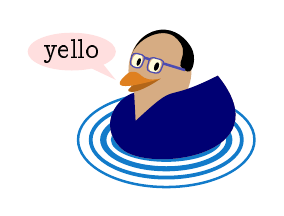
\begin{tikzpicture}[scale=0.8]
  \duck[body=brown!65!white, squareglasses=blue!70!yellow,recedinghair=black,water=cyan!60!blue,speech={yello},bubblecolour=
      pink!50!white,laughing,jacket=blue!45!black]
\end{tikzpicture}
\end{center}
%Load refs.bib file
\bibliographystyle{unsrt} % "IEEE" instead of plain for order of appearnance, not alphabetical
\bibliography{refs} % Entries are in the refs.bib file
\end{document}
